\documentclass{beamer}
\usetheme{metropolis}           % Use metropolis theme
\usepackage{appendixnumberbeamer}
\usepackage{epigraph}
\usepackage{color}
\usepackage{amsopn}
\usepackage{framed}             % for {framed}
\usepackage{tabto}
\graphicspath{{../img/}}

\theoremstyle{definition}
\newtheorem{defn}{Definition}

%%% Bibliography
\usepackage[backend=bibtex, style=authoryear]{biblatex}
\AtBeginBibliography{\tiny}
\bibliography{../src/bibliography.bib}

\setbeamercolor{background canvas}{bg=white}
%\setbeamercolor{title}{fg=white}
%\setbeamercolor{subtitle}{fg=black}
%\setbeamercolor{author}{fg=black}
%\setbeamercolor{institute}{fg=white}

\newcommand{\todo}{\alert{TODO}}
\newcommand{\itemBullet}{\scriptsize$\blacksquare$}
\setbeamertemplate{itemize item}{\itemBullet}
\setbeamertemplate{itemize subitem}{\itemBullet}
\setbeamertemplate{itemize subsubitem}{\itemBullet}
\newcommand{\E}{\mathop{\mathbb{E}}}
\DeclareMathOperator*{\argmax}{arg\,max}
\newcommand{\epiParSpace}{\vskip 1.5ex}
\newcommand{\vect}[1]{\boldsymbol{#1}}
\newcommand{\I}{\mathcal{I}}
\newcommand{\dt}{\tilde{d}}
\newcommand{\It}{\tilde{I}}

\title{Solving Endgames \\in~Large Imperfect-Information Games \\such as~Poker}
\date{September 13, 2016}
\author{Bc.~Karel Ha}
\institute{Department of~Applied Mathematics \\Charles University}

\begin{document}
  \maketitle

  % todo df: subgame / endgame
  % todo application in game playing

  \section{Perfect-Information Subgames}
  % todo Lomonosov chess
  % todo Go CGT
  % todo Go AlphaGo

  \section{Imperfect-Information Subgames}
  % todo df: probabilities, information sets, (imperf-info) subgame
  % todo solving games: sequences, sequence-form LP
  % todo solving games: learning algos
  % todo assumptions: 2-player, we = 1, opponent = 2

  \section{Endgame Solving}
  \begin{frame}{Endgame Solving: Gadget Game}
    \begin{figure}
      \centering
      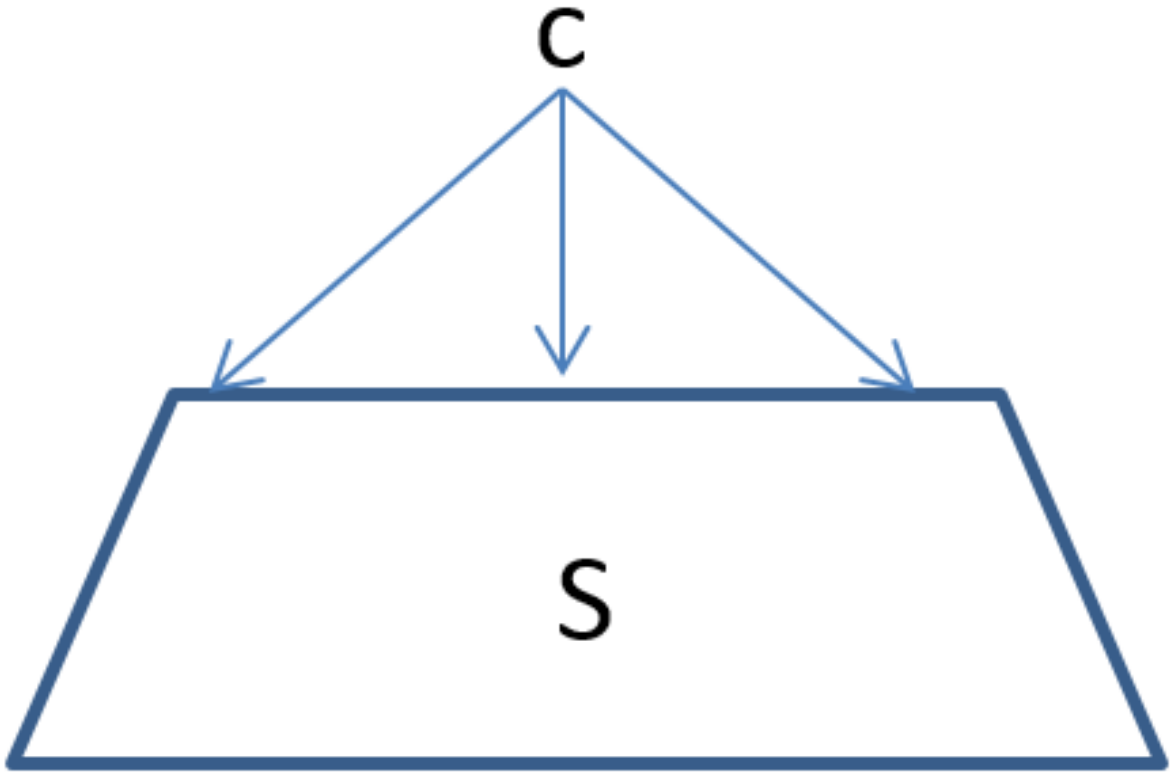
\includegraphics[width=.5\textwidth]{../img/endgame-solving-gadget.png}
    \end{figure}
  \end{frame}

  \begin{frame}{Endgame Solving: Linear Program}
    \begin{equation*}
      \label{lp:endgame-solving}
      \begin{split}
        \max_{v, x}\  f^\top v & \\
        Ex &= e \\
        F^\top v - A^\top x &\le \vect{0} \\
        x &\ge \vect{0}
      \end{split}
    \end{equation*}
  \end{frame}

  \section{CFR-D Decomposition}
  \begin{frame}{CFR-D Decomposition: Gadget Game}
    \begin{figure}[H]
      \centering
      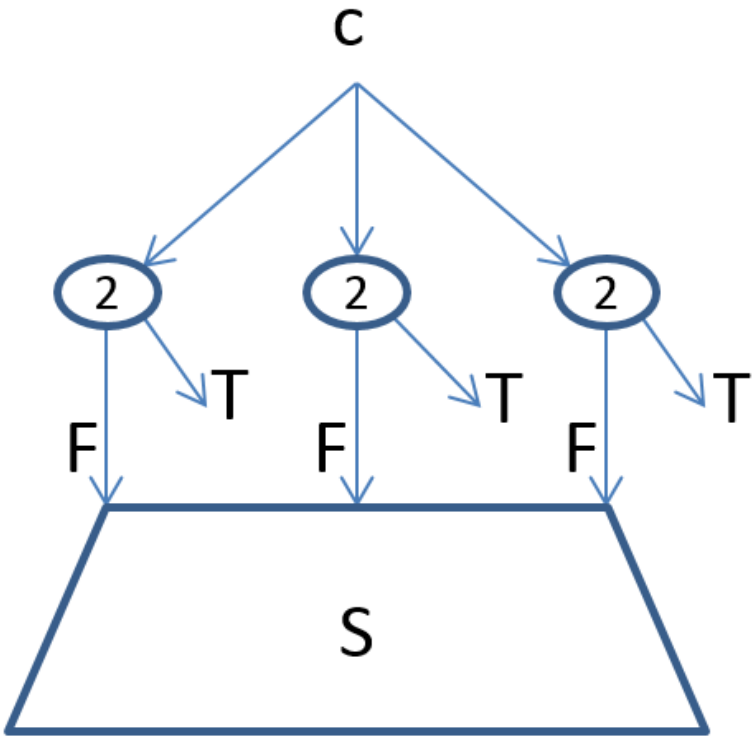
\includegraphics[width=.4\textwidth]{../img/re-solving-game-gadget.png}
    \end{figure}
    \pause

    \begin{itemize}[<+- | alert@+>]
      \item choice of~either to (F)ollow the action into the endgame, or to (T)erminate
      \item utility after the (T)erminal action set to the \emph{counterfactual best-response value}
    \end{itemize}
  \end{frame}

  \begin{frame}{CFR-D Decomposition: Linear Program}
    \begin{equation*}
      \label{lp:cfr-d}
      \begin{split}
        \max_{v, x}\ &0 \\
        \color{red}
        v_I - m &
        \color{red}
        \ge CBV_2^{\sigma_1}(I), \quad I \in \I_2^{R(S)}\\ 
        Ex &= e \\
        F^\top v - A_{\color{red}2}^\top x &\le \vect{0} \\
        x &\ge \vect{0}
      \end{split}
    \end{equation*}
    \pause

    \begin{itemize}[<+- | alert@+>]
      \item $\I_2^{R(S)}$ denotes the root information sets 
      \item $CBV_2^\sigma(I)$ is $2$'s original counterfactual best-response value
    \end{itemize}
  \end{frame}

  \section{Subgame-Margin Maximization}

  \begin{frame}{Subgame-Margin Maximization: Subgame Margin}
    \pause
    \begin{framed}
      Let $\sigma_1$, $\sigma_1'$ be a~pair of~player~$1$'s strategies for subgame~$S$.
      Then a~\alert{subgame margin} is
      \[
        SM_1 (\sigma_1, \sigma_1' , S) =
        \min_{I_2 \in \I_2^{R(S)}}
        \left( CBV_2^{\sigma_1} (I_2) - CBV_2^{\sigma_1'} (I_2) \right)
      \]
    \end{framed}
    \pause

    It measures the ``gap in~decrease'' between the old and the new CBVs, across all root information sets $I_2 \in \I_2^{R(S)}$.
  \end{frame}

  % todo thm: improvement-propto-margin
  \begin{frame}{Subgame-Margin Maximization: Gain Is Proportional to SM}
    \pause
    \begin{theorem}
      Additionally, if there is $\sigma_2^* = BR(\sigma_1')$ such that $\pi^{<\sigma_1',\sigma_2^*>} (I_2) > 0$ for some $I_2 \in\I_2^{R(S)}$, then the gain in~utilities is proportional to SM:
      \[
        u_1(\sigma_1', CBR(\sigma_1')) - u_1(\sigma_1, CBR(\sigma_1)) \ge \pi_{-2}^{\sigma_1'} (I_2) \cdot SM_1(\sigma_1, \sigma_1', S).
      \]
    \end{theorem}
    \pause

    \begin{itemize}[<+- | alert@+>]
       \item ``the probability of~reaching a~subgame'' $\propto \pi_{-2}^{\sigma_1'}(I_2)$
       \item $\uparrow \pi_{-2}^{\sigma_1'}(I_2)$
         \begin{enumerate}[$\Rightarrow$]
           \item $\uparrow$ the bound
           \item $\uparrow$ the probability of~reaching that subgame
         \end{enumerate}
       \item Thus, subgames with larger bounds are likelier to be reached.
    \end{itemize}
  \end{frame}

  \begin{frame}{Subgame-Margin Maximization: Linear Program}
    \begin{equation*}
      \label{lp:max-margin}
      \begin{split}
        \max_{v, x}\ &\textcolor{red}{m} \\
        v_I - m &\ge CBV_2^{\sigma_1}(I), \quad I \in \I_2^{R(S)}\\ 
        Ex &= e \\
        F^\top v - A_2^\top x &\le \vect{0} \\
        x &\ge \vect{0}
      \end{split}
    \end{equation*}
    \pause

    \begin{itemize}[<+- | alert@+>]
      \item $m$ is a~scalar corresponding to the subgame margin
      \item $\approx$ ``gap'' between values $v_I$ and the given constants $CBV_2^\sigma(I)$
      \item \emph{CFR-D Decomposition} only guarantees a~non-negative margin
      \item \emph{Subgame-Margin Maximization} maximizes it
    \end{itemize}
  \end{frame}

  \begin{frame}{Subgame-Margin Maximization: Gadget Game}
    \begin{figure}
      \centering
      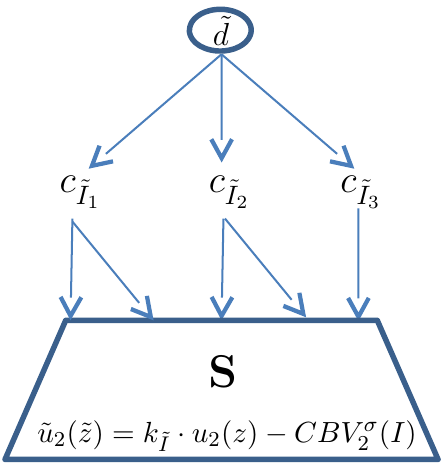
\includegraphics[width=.5\textwidth]{../img/max-margin-gadget.png}
    \end{figure}
    \pause

    Against the original strategy, opponent has a~zero utility at~best.
  \end{frame}


  \section{Ideas for Future Work}

  \begin{frame}{Margins as a~Vector Linear Program}
    \begin{equation*}
      \label{vlp:max-margins}
      \begin{split}
        \max_{v, x}\ &\textcolor{red}{\vect{m}} \\
        v_I - \vect{m}_{\textcolor{red}{I}} &\ge CBV_2^{\sigma_1}(I), \quad I \in \I_2^{R(S)}\\ 
        Ex &= e \\
        F^\top v - A_2^\top x &\le \vect{0} \\
        x &\ge \vect{0}
      \end{split}
    \end{equation*}

    \pause
    \begin{itemize}[<+- | alert@+>]
      \item $\vect{m}_I := CBV_2^{\sigma_1} (I) - CBV_2^{\sigma_1'} (I)$ corresponds to one specific margin
      \item $\vect{m} := (m_I) _{I\in\I_2^{R(S)}}$ is a~vector of~all such margins
      \item multi-criteria optimization problem
      \item corresponding gadget games?
    \end{itemize}
  \end{frame}

  \begin{frame}[standout]
    \begin{center}
      Thank you!
    \end{center}
  \end{frame}

  \begin{frame}[allowframebreaks]{References}
    \tiny
    \printbibliography[heading=none]
  \end{frame}

\end{document}
